\documentclass{article}
\usepackage{graphicx}
\usepackage{float}
\usepackage{fullpage}

\begin{document}

\begin{tabular}{rl}
	\textbf{Lab 9:} & Three Phase Induction Motor\\
	\textbf{Performed:} & April 01, 2013 \\
	\textbf{Partners:} & Rawley Dent \\ & Charles Pittman \\
	\textbf{Instructor:} & Dr.\ Weatherford
\end{tabular}


\section*{Abstract}
	In this experiment, the basic principles of an induction motor were studied.
	Using a wound-rotor motor at two different supply voltages, the motor's
	speed, torque output, and line current was recording at various load torques.

\section*{Results}
	\begin{figure}[H]
		\centering
		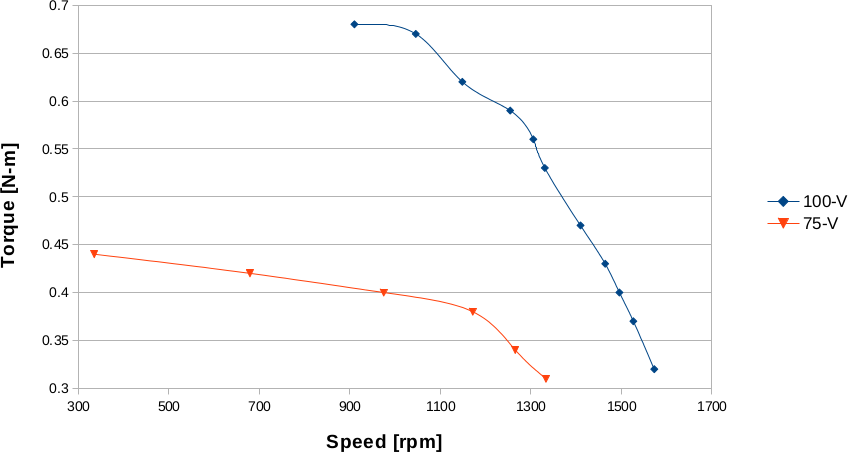
\includegraphics[width=1.0\textwidth]{img/graph}
		\caption{\textbf{Comparison of Output Torque vs. Speed for Different Supply Voltages}}
		\label{fig:graph}
	\end{figure}

\section*{Conclusions}
	In a typical torque speed curve, the plot rises sharply from the starting
	torque to the breakdown (peak) torque, and then decreases linearly to the
	no-load mark. This linear section is the motor's operating region.

	However, the data obtained in the experiment is represented in the figure
	above. The plot is not characteristic of a typical induction motor
	torque-speed curve as described.  This is because of a high unknown rotor
	resistance. Both supply voltages of 100-V and 75-V have the starting torques
	and breakdown torques to be at the same mark. The motor with a starting
	voltage of 100-V has a starting torque of 0.68-Nm and a no-load speed of
	1565-rpm.  The motor with a starting torque of 75-V had a starting torque of
	0.44-Nm and a no-load speed of 1343-rpm. Thus a wound-rotor induction motor
	needs to have a higher supply voltage to be start heavy loads.

\end{document}

